% ============================================================================
% chapitre2.tex — Analyse des besoins
% ============================================================================
\chapter{Analyse des besoins}
\label{chap:besoins}

\introchapitre

Ce chapitre presente l'analyse des besoins du systeme a concevoir. Nous distinguons
les besoins fonctionnels, organises par couche architecturale, des besoins non
fonctionnels qui definissent les exigences de qualite du systeme. Nous concluons par
la modelisation des cas d'utilisation.

\section{Besoins fonctionnels}
\label{sec:besoins-fonc}

\subsection{Couche ingestion --- Apache Kafka}

\begin{itemize}
    \item Recevoir en continu les transactions de paiement chiffrees, provenant des
    canaux \texttt{SO\_CARTE} et \texttt{SO\_MOBILE},
    \item Chiffrer chaque transaction avec l'algorithme Fernet avant publication dans
    le topic Kafka \texttt{payments}, le numero de carte etant masque selon la norme
    PCI-DSS,
    \item Maintenir les sept topics du pipeline (\texttt{payments},
    \texttt{payments.decrypted}, \texttt{payments.validated},
    \texttt{payments.normalized}, \texttt{payments.gold}, \texttt{payments.gold.flat}
    et \texttt{payments.dlq}) avec une politique de retention explicite par topic.
\end{itemize}

\subsection{Couche traitement --- Apache Flink}

\begin{itemize}
    \item \textbf{Job 1 --- Decryptage} : dechiffrer le payload Fernet de chaque
    message et ecrire l'enregistrement brut dans la couche Bronze de MinIO ; tout
    echec de decryptage est route vers la DLQ,
    \item \textbf{Job 2 --- Validation} : appliquer en une seule passe 9 regles de
    validation sur chaque transaction decryptee --- 6 regles metier HPS
    (\texttt{MESSAGE\_TYPE}, \texttt{TRANSACTION\_AMOUNT}, \texttt{TRANSACTION\_CURRENCY},
    \texttt{ISSUING\_BANK}, \texttt{CARD\_TYPE}, \texttt{REJECT\_CODE}) et 3 regles de
    conformite bancaire ISO~8583 (MTI reconnu), ISO~4217 (devise valide) et ISO~7812
    (algorithme de Luhn sur le PAN),
    \item \textbf{Job 3 --- Normalisation et enrichissement} : normaliser les formats
    de date et de montant, et enrichir chaque enregistrement (\texttt{processed\_at},
    \texttt{source\_system}, \texttt{pipeline\_version}, \texttt{card\_scheme},
    \texttt{mti\_name}, \texttt{currency\_alpha}, \texttt{mcc\_description}),
    \item \textbf{Job 4 --- Optimisation} : dedupliquer les transactions par
    \texttt{AUTHORIZATION\_CODE} via un etat Flink distribue, router chaque
    transaction selon son canal de paiement, attribuer un score de risque
    (\texttt{HIGH}/\texttt{MEDIUM}/\texttt{LOW}) et publier le resultat dans
    \texttt{payments.gold}.
\end{itemize}

\subsection{Couche stockage --- MinIO (architecture Medallion)}

\begin{itemize}
    \item \textbf{Bronze} : donnees brutes decryptees, conservees pour l'audit et le
    rejeu,
    \item \textbf{Silver} : donnees validees, normalisees et enrichies,
    \item \textbf{Gold} : donnees finales dedupliquees, scorees et routees par canal,
    \item \textbf{DLQ} : transactions invalides ou non traitables, avec leur motif de
    rejet, sans aucune donnee sensible.
\end{itemize}

\subsection{Couche persistance finale --- Kafka Connect JDBC Sink}

\begin{itemize}
    \item Republier chaque enregistrement \texttt{payments.gold} sous forme d'un
    message a schema explicite dans le topic intermediaire
    \texttt{payments.gold.flat} (composant \texttt{gold-flattener}),
    \item Alimenter automatiquement et en temps reel la table relationnelle
    \texttt{gold\_transactions} de PostgreSQL via le connecteur Kafka Connect JDBC Sink
    (Debezium), en mode \textit{upsert} sur la cle \texttt{authorization\_code},
    \item Permettre l'interrogation SQL de \texttt{gold\_transactions} pour des
    analyses sur les scores de risque, les canaux de paiement et les tendances
    temporelles.
\end{itemize}

\subsection{Couche monitoring}

\begin{itemize}
    \item Exposer des metriques temps reel sur chaque etape du pipeline (profondeur
    des topics Kafka, objets MinIO par couche, lignes \texttt{gold\_transactions},
    repartition par score de risque et par canal),
    \item Collecter ces metriques via Prometheus et les restituer dans des tableaux
    de bord Grafana actualises automatiquement.
\end{itemize}

\section{Besoins non fonctionnels}
\label{sec:besoins-nonfonc}

\begin{itemize}
    \item \textbf{Fiabilite} : Apache Flink est configure avec un mecanisme de
    checkpointing en mode \texttt{EXACTLY\_ONCE}, garantissant la reprise automatique
    apres une panne sans perte ni duplication de donnees,
    \item \textbf{Scalabilite} : l'architecture Kubernetes permet de faire evoluer
    horizontalement le nombre de TaskManagers Flink et de repliques Kafka selon la
    charge,
    \item \textbf{Securite} : chiffrement Fernet (AES-128-CBC + HMAC-SHA256) de
    toutes les donnees de transaction avant publication dans Kafka, masquage
    systematique du numero de carte, isolation des composants par Network Policies
    Kubernetes et gestion des secrets via Kubernetes Secrets,
    \item \textbf{Observabilite} : huit tableaux de bord Grafana couvrant
    l'infrastructure, le pipeline Flink, Kafka, MinIO et les metriques metier
    personnalisees,
    \item \textbf{Maintenabilite} : infrastructure entierement definie en Infrastructure
    as Code via Terraform, garantissant la reproductibilite des deploiements,
    \item \textbf{Non-interference avec l'existant} : le pipeline temps reel est
    deploye dans des namespaces Kubernetes isoles, sans aucune modification ni
    interaction avec les systemes de production existants,
    \item \textbf{Portabilite} : solution validee sur Minikube en environnement de
    developpement, transposable vers un cluster Kubernetes manage (ex. AKS) sans
    modification du code applicatif.
\end{itemize}

\section{Modelisation des cas d'utilisation}
\label{sec:uc}

\subsection{Acteurs du systeme}

Le diagramme de cas d'utilisation global modelise les interactions entre les
differents acteurs du systeme et les fonctionnalites offertes par la plateforme. Le
tableau \ref{tab:acteurs} identifie ces acteurs et leurs responsabilites principales.

\begin{table}[H]
\centering
\renewcommand{\arraystretch}{1.5}
\begin{tabular}{|l|p{11.5cm}|}
\hline
\textbf{Acteur} & \textbf{Responsabilites principales} \\
\hline
\textbf{Data Engineer} &
\begin{itemize}
    \item Configurer et lancer le producteur Python qui lit et chiffre les
    transactions depuis la source CSV,
    \item Deployer et soumettre les quatre jobs Flink de traitement,
    \item Gerer les topics Kafka, les connecteurs Kafka Connect et le composant
    \texttt{gold-flattener} alimentant le Data Mart,
    \item Surveiller le pipeline via Grafana et l'exporteur de metriques metier.
\end{itemize} \\
\hline
\textbf{Administrateur} &
\begin{itemize}
    \item Deployer et gerer l'infrastructure via Terraform,
    \item Surveiller l'etat des jobs via le tableau de bord Flink,
    \item Consulter les donnees dans la console MinIO et gerer les topics Kafka,
    \item Gerer les connecteurs Kafka Connect (source et sink).
\end{itemize} \\
\hline
\textbf{Data Analyste} &
\begin{itemize}
    \item Interroger la table \texttt{gold\_transactions} via SQL pour des analyses
    metier en temps reel,
    \item Consulter les scores de risque et les canaux de paiement,
    \item Visualiser les tableaux de bord Grafana alimentes en continu par le
    pipeline.
\end{itemize} \\
\hline
\end{tabular}
\caption{Acteurs et responsabilites dans la plateforme de streaming temps reel}
\label{tab:acteurs}
\end{table}

\subsection{Diagramme global}

La figure \ref{fig:useGlob} presente le diagramme de cas d'utilisation global de la
plateforme.

\begin{figure}[H]
\centering
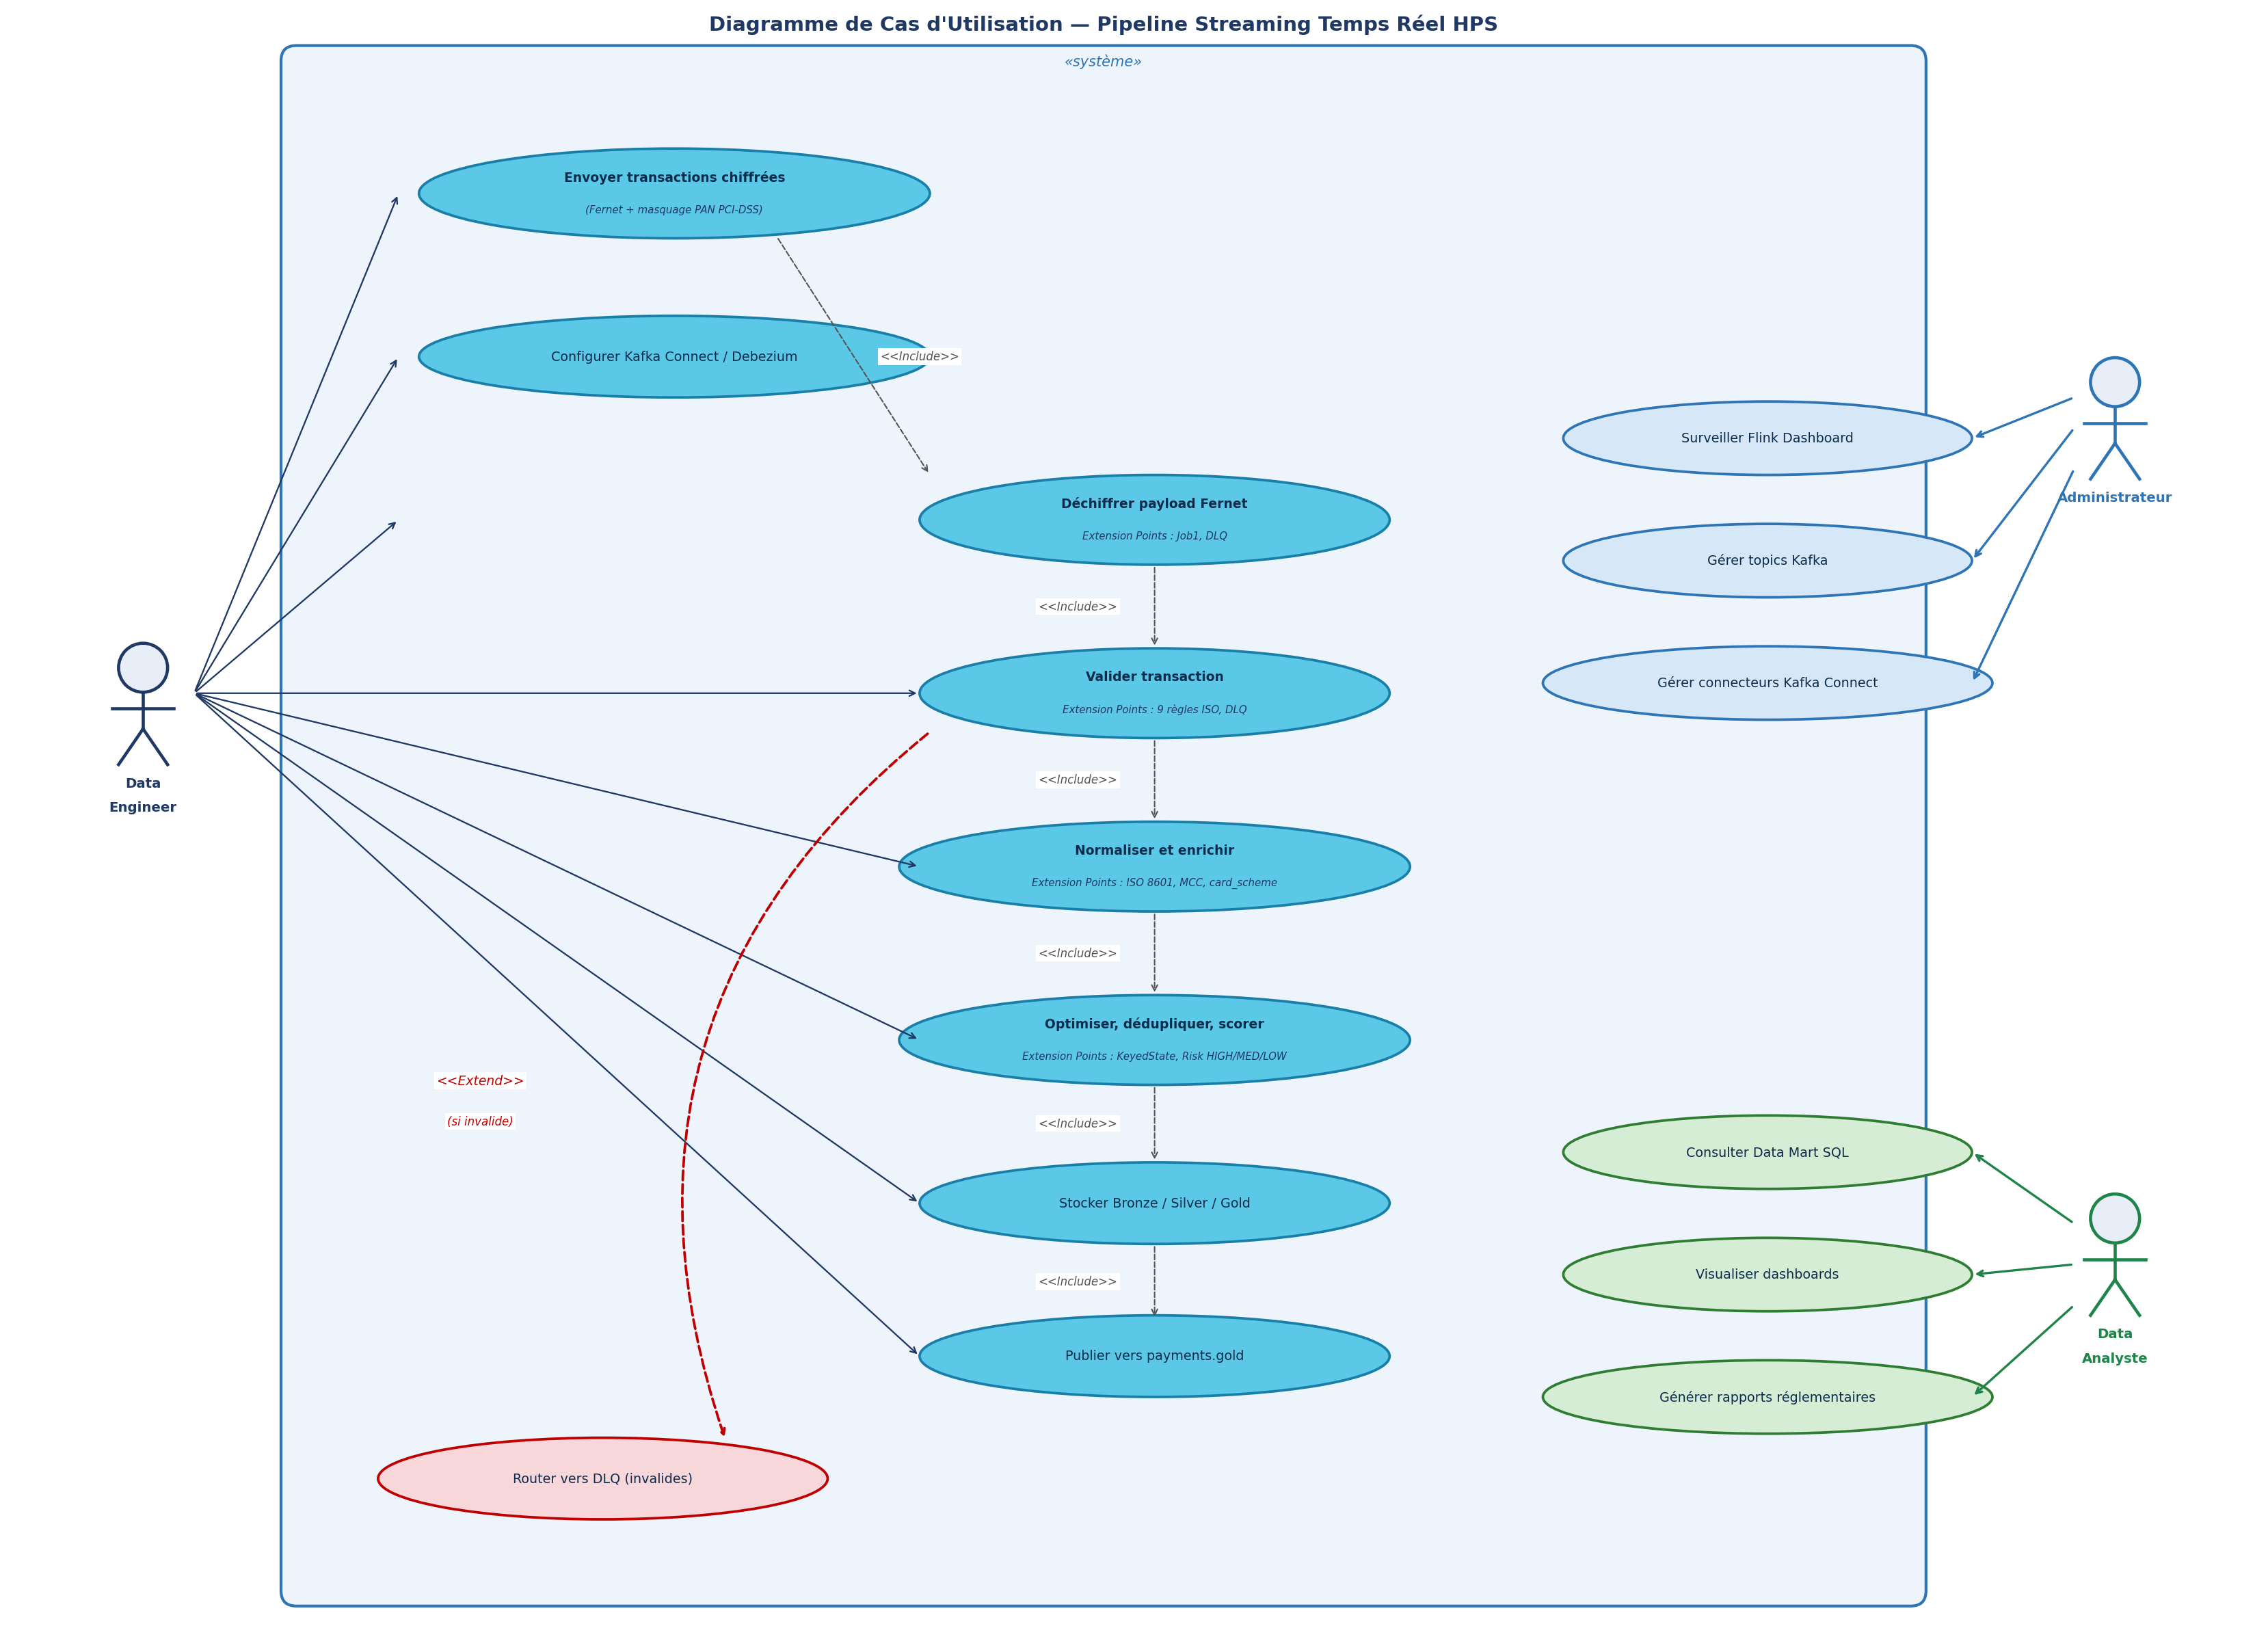
\includegraphics[width=\textwidth]{figures/useCaseGlobal_v3.png}
\caption{Diagramme de cas d'utilisation global de la plateforme de streaming}
\label{fig:useGlob}
\end{figure}

\subsection{Description textuelle des cas d'utilisation principaux}

Le cas d'utilisation \textit{« Surveiller le pipeline »} permet a l'administrateur et
au Data Engineer de consulter, a tout moment, l'etat de chaque composant (jobs Flink
en cours d'execution, profondeur des topics Kafka, statut des connecteurs Kafka
Connect) via les tableaux de bord Grafana. Le cas d'utilisation \textit{« Interroger
les donnees Gold »} permet au Data Analyste d'executer des requetes SQL sur la table
\texttt{gold\_transactions} afin d'en extraire des indicateurs metier (volume par
score de risque, repartition par canal de paiement). Le cas d'utilisation
\textit{« Deployer l'infrastructure »} permet a l'administrateur de provisionner ou de
mettre a jour l'ensemble du cluster en executant \texttt{terraform apply}, de maniere
idempotente et reproductible.

\conclusionchapitre

Ce chapitre a precise les besoins fonctionnels et non fonctionnels du systeme, organises
par couche architecturale, ainsi que les acteurs et leurs interactions avec la
plateforme. Le chapitre suivant traduit ces besoins en une conception detaillee, tant
dynamique que statique et architecturale.
